% =====================================================================
%  Detector de Vazamento de Gás com MSP430
%  Relatório do Projeto Final — Laboratório de Sistemas Microprocessados
%  Universidade de Brasília — Faculdade de Tecnologia
%
%  Compilar de dentro desta pasta:
%    C:\texlive\2025\bin\windows\pdflatex.exe -interaction=nonstopmode relatorio.tex
%  (rodar duas vezes para acertar o sumário)
% =====================================================================
\documentclass[11pt,a4paper]{article}

% ---------- codificação e idioma ----------
\usepackage[T1]{fontenc}
\usepackage[utf8]{inputenc}
\usepackage[brazil]{babel}
\usepackage{textcomp}

% ---------- layout ----------
\usepackage[a4paper,top=2.6cm,bottom=2.6cm,left=2.8cm,right=2.8cm]{geometry}
\usepackage{indentfirst}
\usepackage{microtype}

% ---------- matemática, figuras e tabelas ----------
\usepackage{amsmath}
\usepackage{graphicx}
\usepackage{booktabs}
\usepackage{array}
\usepackage{caption}
\usepackage{xcolor}

% ---------- links ----------
\usepackage[hidelinks]{hyperref}
\hypersetup{
  pdftitle={Detector de Vazamento de Gas com MSP430},
  pdfauthor={Victor Hugo Guimaraes Nascimento; Davi Sousa da Vinha},
  pdfsubject={Relatorio do Projeto Final - Laboratorio de Sistemas Microprocessados},
  pdfkeywords={MSP430, MSP430F5529, MQ-2, ADC12, LCD 16x2, buzzer, deteccao de gas}
}

% ---------- caminho das figuras ----------
\graphicspath{{../docs/figures/original/}}

% ---------- numeração das equações por seção ----------
\numberwithin{equation}{section}

% ---------- legendas ----------
\captionsetup{font=small,labelfont=bf,skip=6pt}

\begin{document}

% =====================================================================
%  CAPA
% =====================================================================
\begin{titlepage}
  \centering
  {\large Universidade de Brasília\par}
  \vspace{2pt}
  {\large Faculdade de Tecnologia\par}
  \vspace{2pt}
  {\large Departamento de Engenharia Elétrica\par}
  \vspace{2pt}
  {\large Laboratório de Sistemas Microprocessados\par}

  \vspace{1.8cm}
  {\large Professor: José Edil G. de Medeiros\par}

  \vspace{2.4cm}
  {\Huge\bfseries Detector de Vazamento de Gás com MSP430\par}

  \vspace{0.9cm}
  {\large\itshape Relatório do Projeto Final\par}

  \vspace{2.6cm}
  {\large Victor Hugo Guimarães Nascimento\par}
  \vspace{4pt}
  {\large Davi Sousa da Vinha\par}

  \vfill
  {\large Brasília\par}
  {\large 2026/1\par}
\end{titlepage}

% =====================================================================
%  RESUMO / NOTA
% =====================================================================
\begin{center}
  \begin{minipage}{0.86\textwidth}
    \small
    \textbf{Resumo.} Este relatório documenta o projeto final da disciplina de Laboratório de
    Sistemas Microprocessados: um detector de vazamento de gás de baixo custo baseado na LaunchPad
    MSP430F5529LP, no sensor MQ-2, em um display LCD 16x2 e em alertas sonoro e visual. O trabalho
    parte de uma pesquisa de campo com moradores de um condomínio residencial, define o problema a
    partir dos dados coletados, propõe uma arquitetura embarcada e detalha a implementação:
    conversão A/D do sinal do sensor, cálculo do percentual em relação ao limite calibrado,
    temporização por timer, acionamento do buzzer por PWM e silenciamento temporário pelo botão da
    própria placa.
  \end{minipage}
\end{center}

\vspace{0.6cm}

\tableofcontents
\newpage

% =====================================================================
%  CAPÍTULO 1
% =====================================================================
\section{Pesquisa de Campo}
\label{cap:pesquisa}

\subsection{Contextualização}

A pesquisa de campo foi planejada para sondar situações de risco doméstico percebidas por moradores
de um ambiente residencial, especialmente idosos, familiares, cuidadores e pessoas responsáveis por
atividades domésticas.

Situações de risco doméstico fazem parte do cotidiano de muitas pessoas e podem ocorrer por
distração, esquecimento, dificuldade de percepção de sinais de perigo ou ausência de mecanismos
automáticos de alerta. Esses problemas podem se tornar mais relevantes em ambientes onde vivem
idosos, pessoas com limitações sensoriais ou moradores que passam grande parte do tempo sozinhos.

Entretanto, muitas dessas situações acabam sendo percebidas apenas após acidentes, falhas ou relatos
de terceiros, tornando importante investigar quais problemas domésticos afetam mais a comunidade e
como os moradores lidam com questões relacionadas à segurança no cotidiano.

\subsection{Comunidade pesquisada}

A comunidade escolhida foi o condomínio onde o pesquisador reside. O público previsto incluiu idosos,
moradores que vivem sozinhos, cuidadores, familiares responsáveis por idosos e moradores que já
passaram por situações de risco doméstico.

Esse público foi escolhido por estar diretamente relacionado ao contexto investigado e por poder
relatar experiências, dificuldades e preocupações relacionadas à segurança em ambientes residenciais.

\subsection{Justificativa da escolha}

A escolha dessa comunidade se justifica pela proximidade com o cotidiano investigado e pela
possibilidade de compreender problemas reais enfrentados pelos moradores. Além disso, a presença de
idosos e pessoas que vivem sozinhas pode permitir identificar situações em que dificuldades de
percepção, distração ou ausência de mecanismos de alerta contribuam para aumentar riscos domésticos.

A pesquisa com essa comunidade permite compreender melhor quais situações são consideradas mais
preocupantes pelos moradores e quais necessidades podem existir relacionadas à segurança doméstica.

\subsection{Objetivo da pesquisa de campo}

O objetivo da pesquisa de campo foi investigar como moradores de ambientes residenciais percebem
situações de risco doméstico e identificar dificuldades relacionadas à segurança no cotidiano.

Mais especificamente, a pesquisa buscou:

\begin{itemize}
  \item compreender quais situações domésticas são consideradas mais perigosas pelos moradores;
  \item investigar se os moradores já passaram por acidentes, falhas ou situações de risco doméstico;
  \item identificar dificuldades relacionadas à percepção de problemas domésticos;
  \item compreender como os moradores lidam com situações de risco no dia a dia;
  \item levantar possíveis necessidades da comunidade que pudessem motivar uma solução embarcada.
\end{itemize}

\subsection{Método de pesquisa}

Inicialmente, foram previstas entrevistas curtas e conversas informais com moradores do condomínio.
As perguntas planejadas abordavam situações de risco doméstico, acidentes dentro de casa, percepção de
perigo, maior vulnerabilidade de idosos e utilidade de mecanismos automáticos de alerta.

As respostas seriam analisadas para identificar padrões, preocupações recorrentes e possíveis
necessidades relacionadas à segurança doméstica. A expectativa era que os resultados permitissem
definir com mais precisão um problema real da comunidade e orientar as próximas etapas do projeto.

% =====================================================================
%  CAPÍTULO 2
% =====================================================================
\section{Entrevistas e Levantamento de Necessidades}
\label{cap:entrevistas}

\subsection{Relato identificado na comunidade}

Durante as conversas realizadas com moradores, uma moradora relatou possuir dificuldade para perceber
cheiro de gás. Segundo o relato, houve um vazamento no fogão de sua residência que permaneceu sem
identificação durante determinado período.

A situação só foi percebida após a troca do botijão, quando o responsável pela instalação identificou
forte cheiro de gás no ambiente e alertou sobre a existência do vazamento.

O caso chamou atenção por evidenciar que a identificação de vazamentos pode depender fortemente da
percepção humana, especialmente do olfato.

Esse relato indicou uma possível vulnerabilidade em ambientes residenciais, principalmente em
situações envolvendo idosos, pessoas com limitações sensoriais, distração ou ausência de pessoas
próximas ao local do vazamento.

\subsection{Ampliação da pesquisa por formulário digital}

A partir desse relato, o tema foi aprofundado por meio de um formulário digital na plataforma Tally.
O formulário foi compartilhado com moradores do condomínio e também com pessoas externas à comunidade
inicial, buscando obter uma visão mais ampla sobre hábitos de segurança, percepção de risco e
preferências de alerta em situações relacionadas ao uso de gás de cozinha.

As perguntas utilizadas no formulário foram:

\begin{enumerate}
  \item Você utiliza botijão de gás ou gás encanado?
  \item Qual é a sua idade?
  \item Com que frequência você utiliza o fogão a gás?
  \item Você já presenciou ou suspeitou de algum vazamento de gás?
  \item Como você identificaria um possível vazamento de gás?
  \item Você possui algum detector ou sistema automático de alerta de gás?
  \item Você considera que apenas o cheiro do gás é suficiente para perceber um vazamento?
  \item Em uma situação de vazamento, qual tipo de alerta seria mais útil?
  \item Você acha muito importante que o alarme seja alto o suficiente para ser ouvido em outros cômodos?
  \item Um botão para silenciar temporariamente o alarme seria útil?
  \item Onde você acha que um dispositivo de alerta de gás deveria ser instalado?
  \item Quais características seriam mais importantes em um sistema desse tipo?
\end{enumerate}

\subsection{Resultados obtidos}

\subsubsection{Perfil de uso do gás}

A maioria dos participantes informou utilizar botijão de gás. Além disso, a maior parte afirmou
utilizar o fogão a gás várias vezes ao dia, indicando que o tema está relacionado a uma atividade
cotidiana e recorrente.

% --- figuras 2.1 a 2.11 (numeração do relatório original) ---
\setcounter{figure}{0}
\renewcommand{\thefigure}{2.\arabic{figure}}

\begin{figure}[htbp]
  \centering
  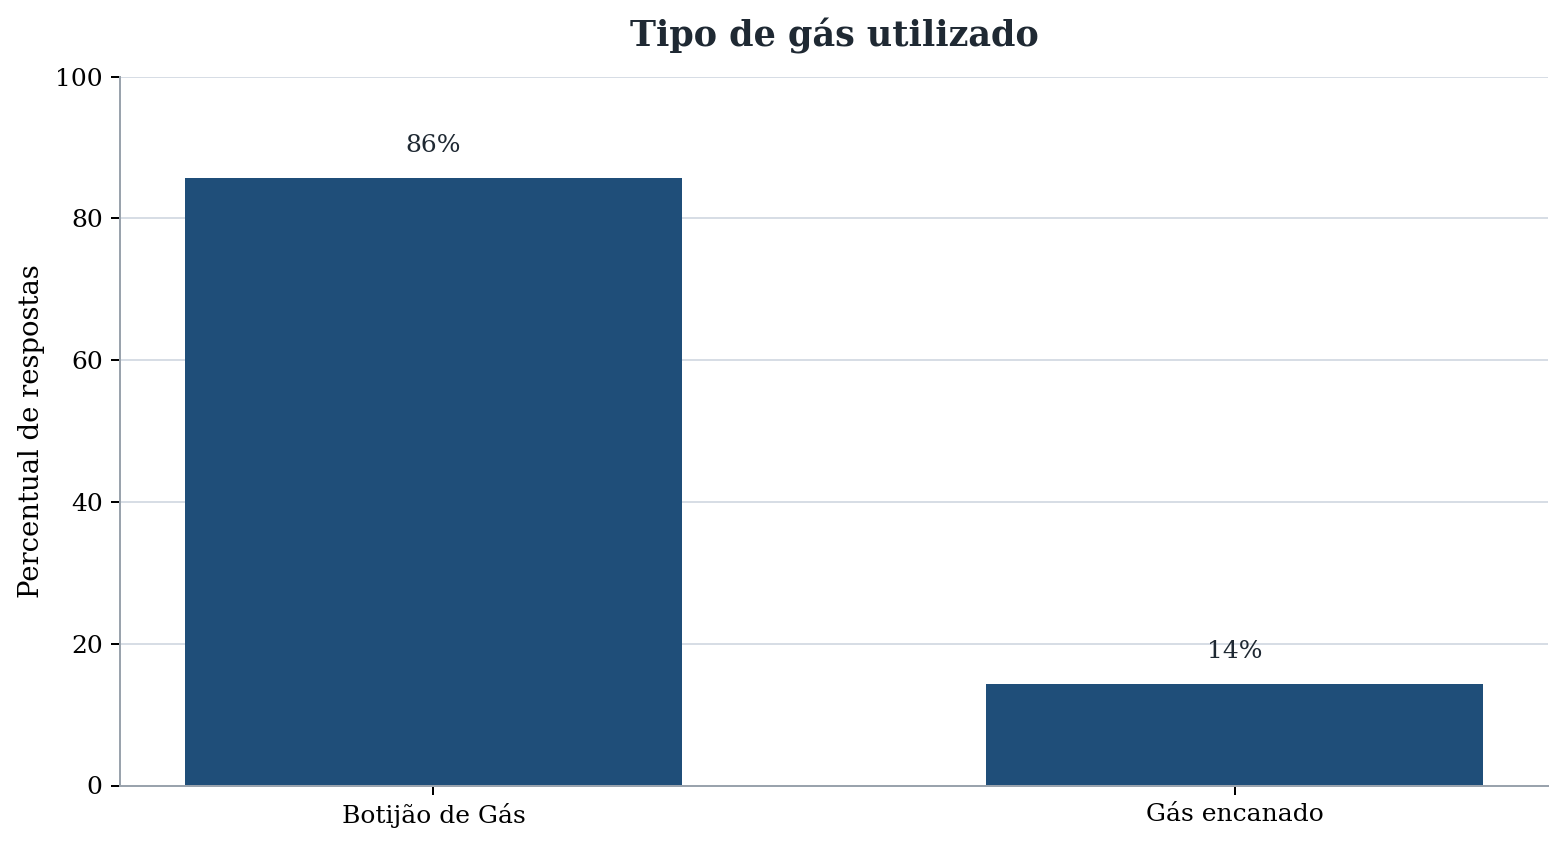
\includegraphics[width=0.78\textwidth]{figura-2.1.png}
  \caption{Tipo de gás utilizado pelos participantes.}
  \label{fig:2.1}
\end{figure}

\begin{figure}[htbp]
  \centering
  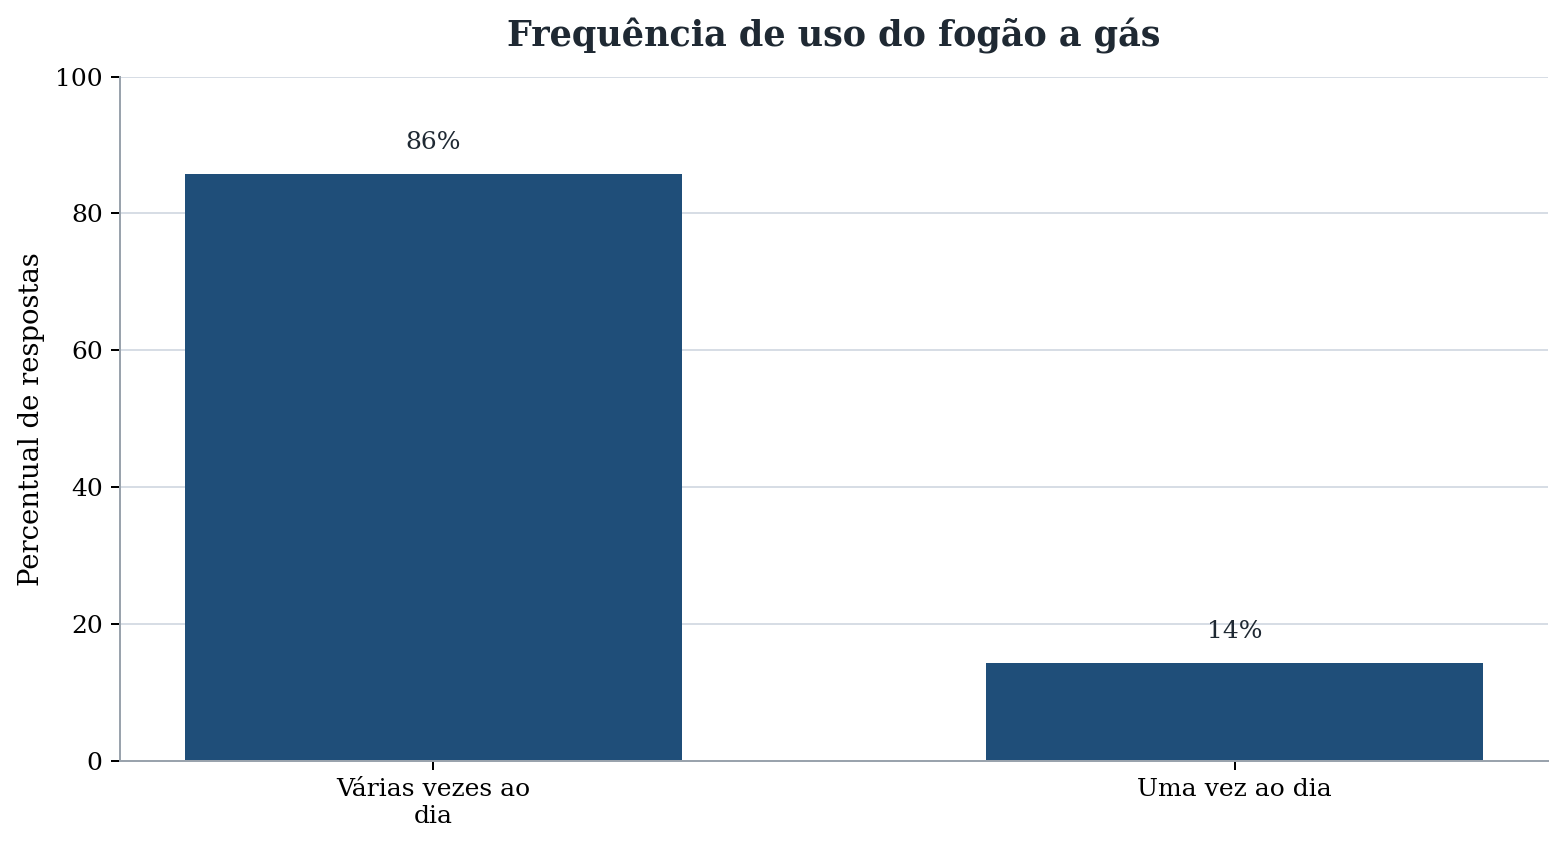
\includegraphics[width=0.78\textwidth]{figura-2.2.png}
  \caption{Frequência de uso do fogão a gás.}
  \label{fig:2.2}
\end{figure}

\subsubsection{Experiência com vazamentos e mecanismos de detecção}

Os dados indicam que uma parte significativa dos participantes já presenciou ou suspeitou de algum
vazamento de gás. Ao mesmo tempo, quase todos afirmaram não possuir detector ou sistema automático de
alerta, o que reforça a dependência de métodos manuais ou sensoriais para identificar situações de
risco.

\begin{figure}[htbp]
  \centering
  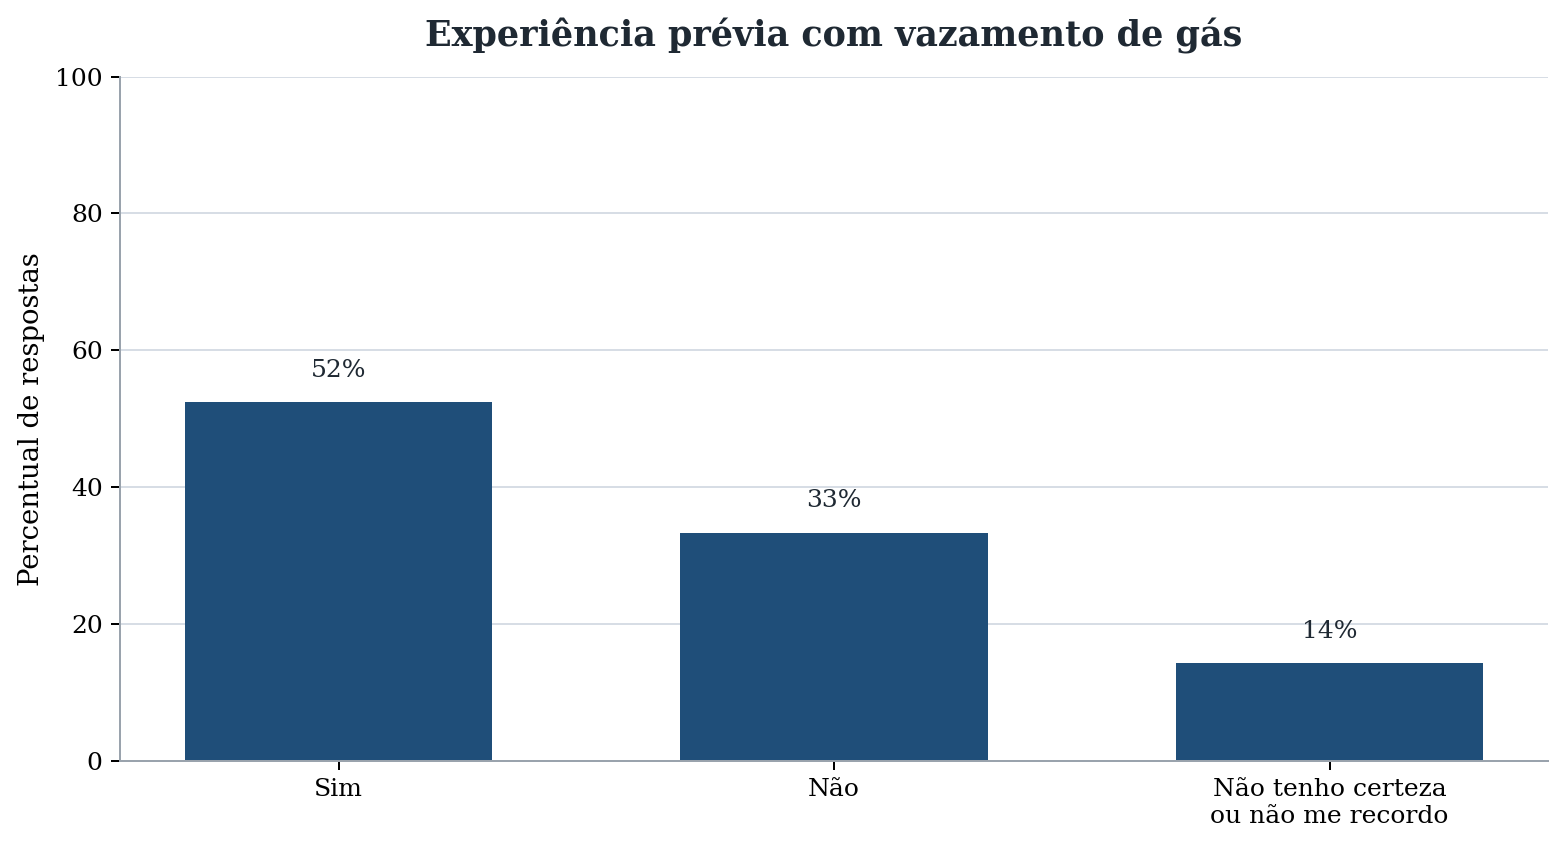
\includegraphics[width=0.78\textwidth]{figura-2.3.png}
  \caption{Experiência prévia com suspeita ou vazamento de gás.}
  \label{fig:2.3}
\end{figure}

\begin{figure}[htbp]
  \centering
  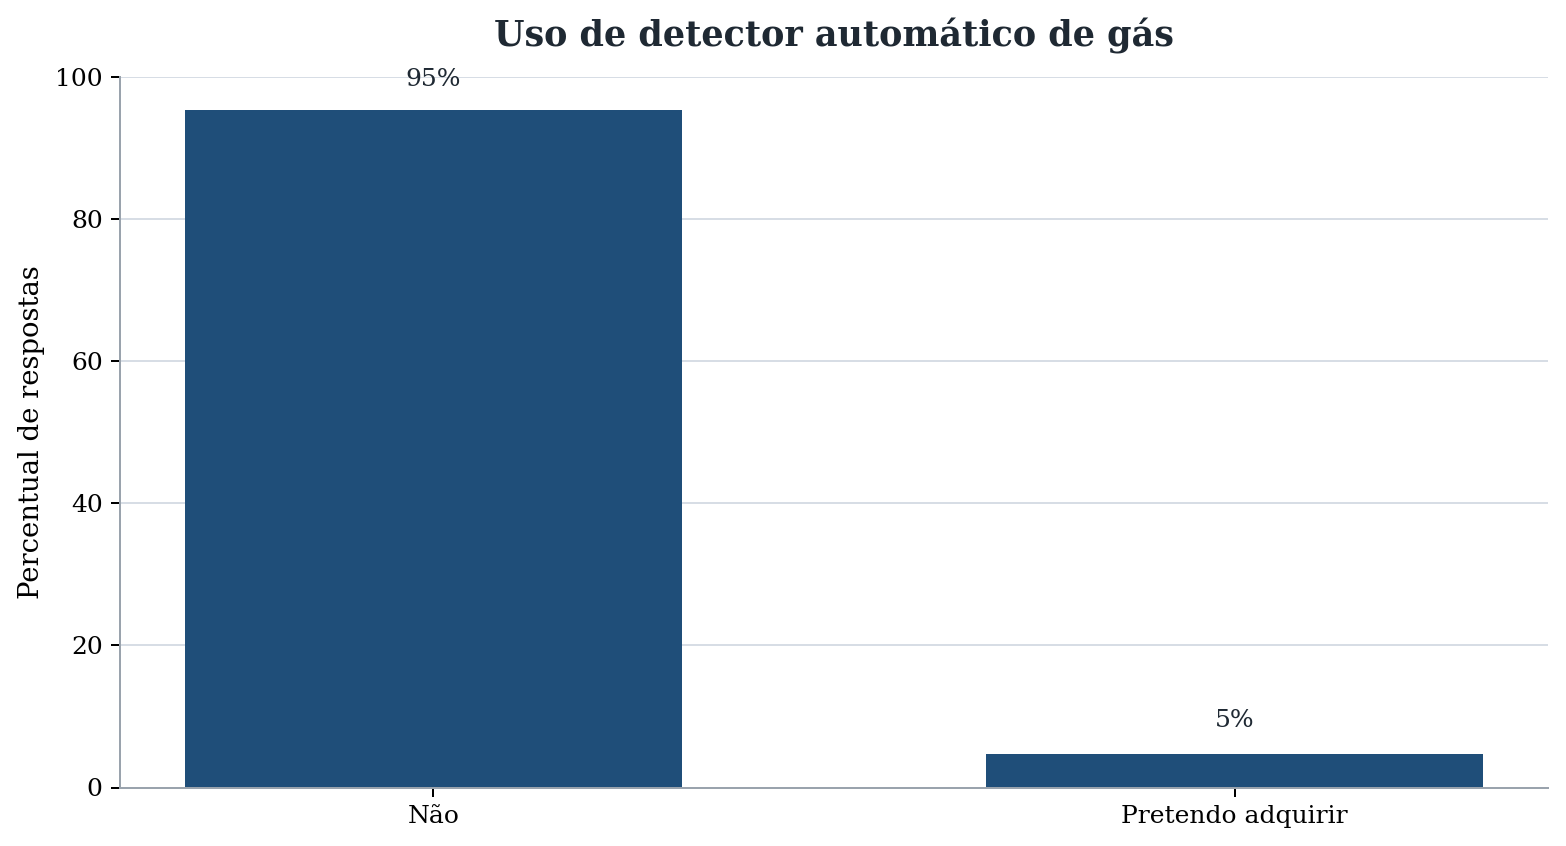
\includegraphics[width=0.78\textwidth]{figura-2.4.png}
  \caption{Uso de detector ou sistema automático de alerta.}
  \label{fig:2.4}
\end{figure}

\subsubsection{Dependência da percepção humana}

Todos os participantes indicaram o cheiro como forma de identificar um possível vazamento. Entretanto,
nem todos consideram que apenas o cheiro é suficiente em qualquer situação. Esse resultado reforça o
problema identificado no relato da moradora, pois mostra que a detecção ainda depende fortemente da
percepção humana.

\begin{figure}[htbp]
  \centering
  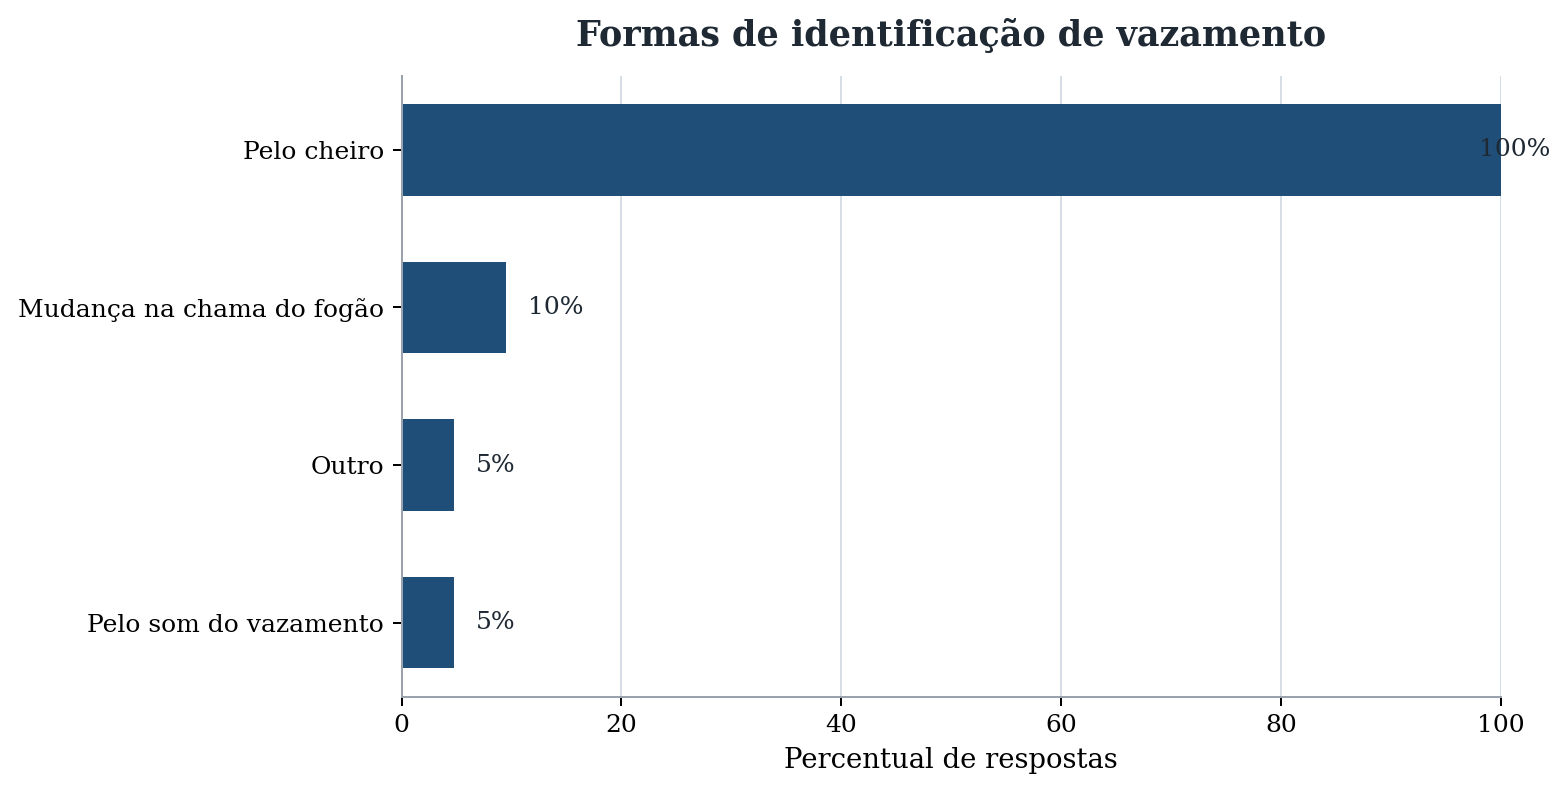
\includegraphics[width=0.78\textwidth]{figura-2.5.png}
  \caption{Formas de identificação de possível vazamento.}
  \label{fig:2.5}
\end{figure}

\begin{figure}[htbp]
  \centering
  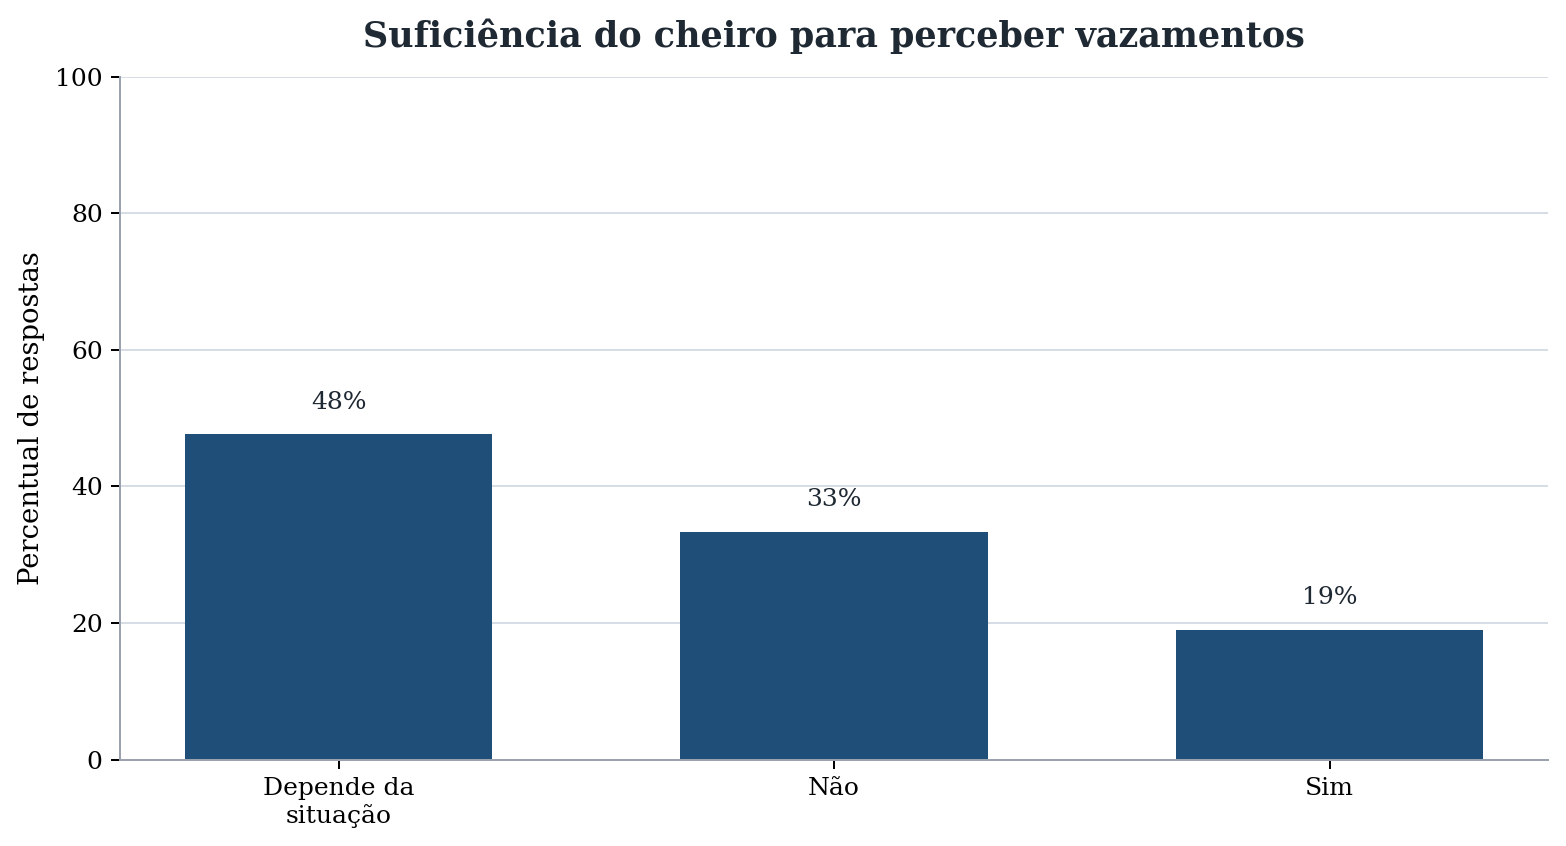
\includegraphics[width=0.78\textwidth]{figura-2.6.png}
  \caption{Percepção sobre a suficiência do cheiro para detectar vazamentos.}
  \label{fig:2.6}
\end{figure}

\subsubsection{Preferências de alerta}

As respostas indicaram interesse por alertas sonoros, visuais e combinações de diferentes formas de
aviso. A maioria também considerou importante que o alarme seja perceptível em outros cômodos da
residência.

\begin{figure}[htbp]
  \centering
  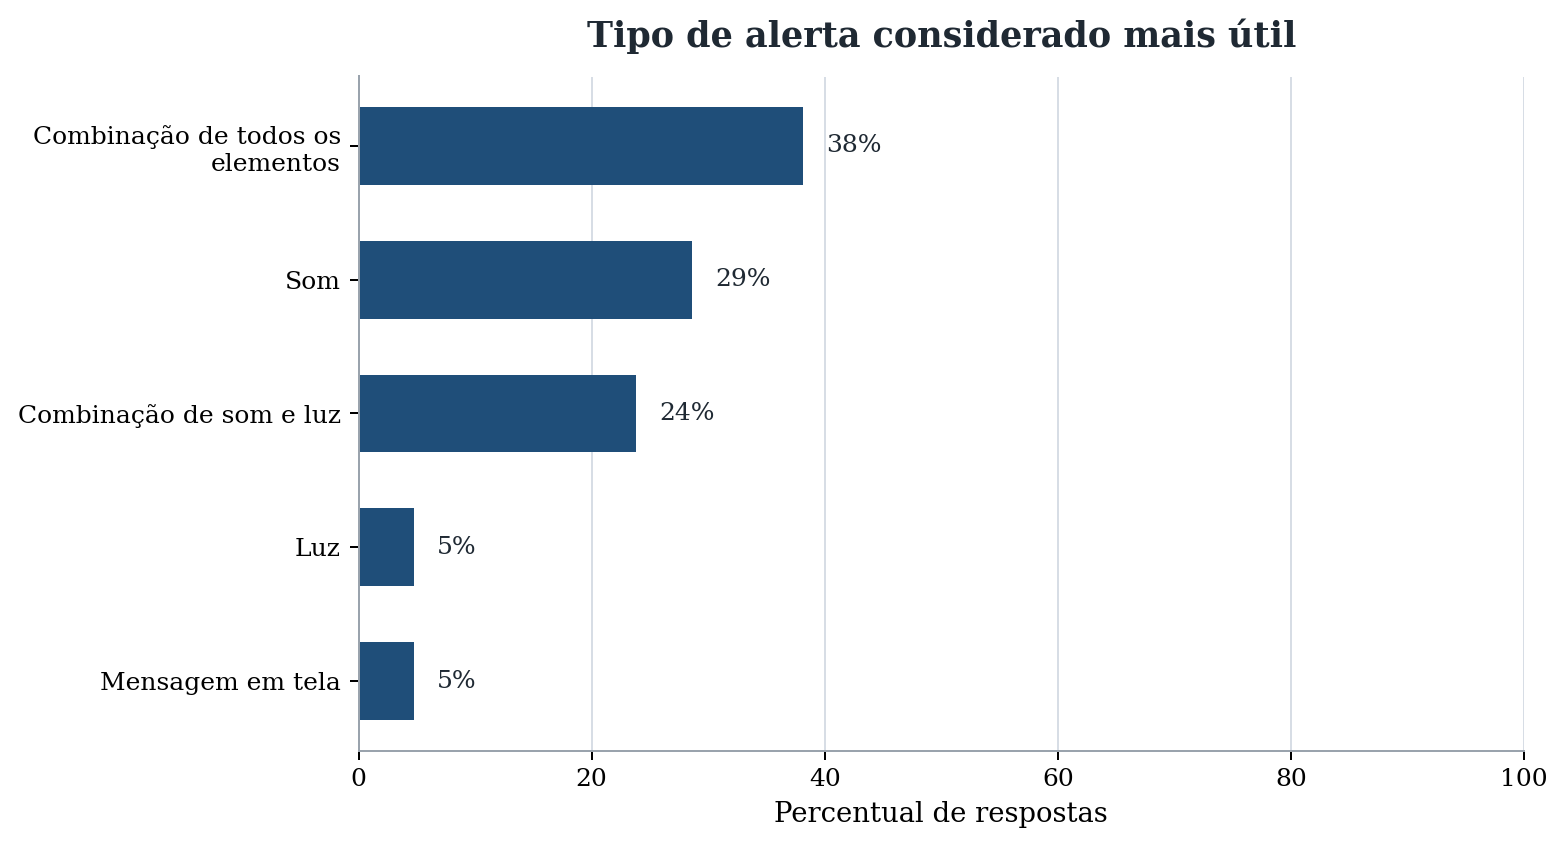
\includegraphics[width=0.78\textwidth]{figura-2.7.png}
  \caption{Tipos de alerta considerados mais úteis.}
  \label{fig:2.7}
\end{figure}

\begin{figure}[htbp]
  \centering
  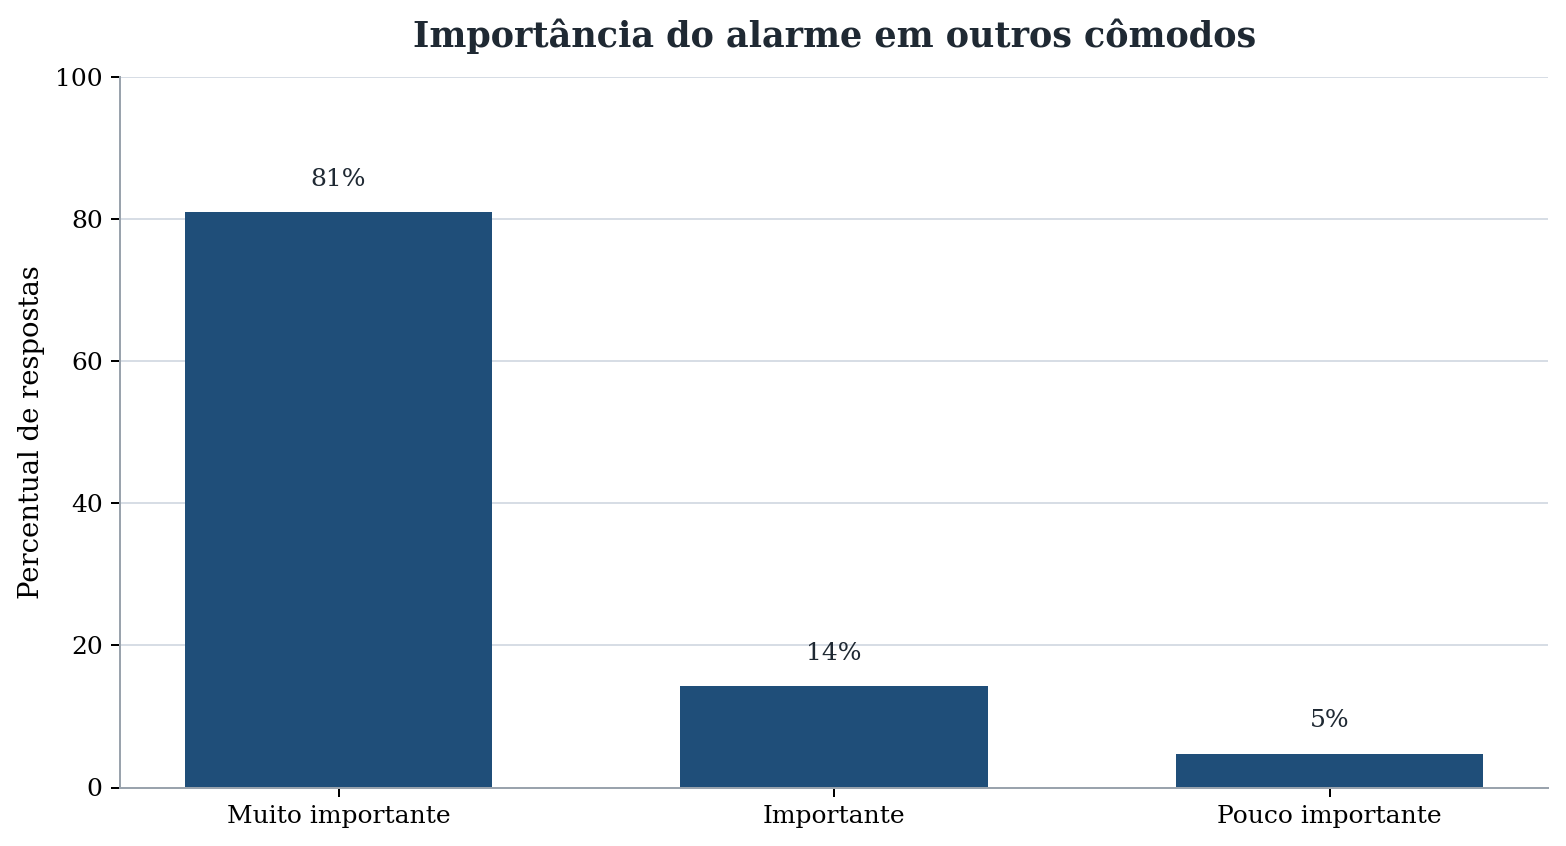
\includegraphics[width=0.78\textwidth]{figura-2.8.png}
  \caption{Importância de o alarme ser ouvido em outros cômodos.}
  \label{fig:2.8}
\end{figure}

\begin{figure}[htbp]
  \centering
  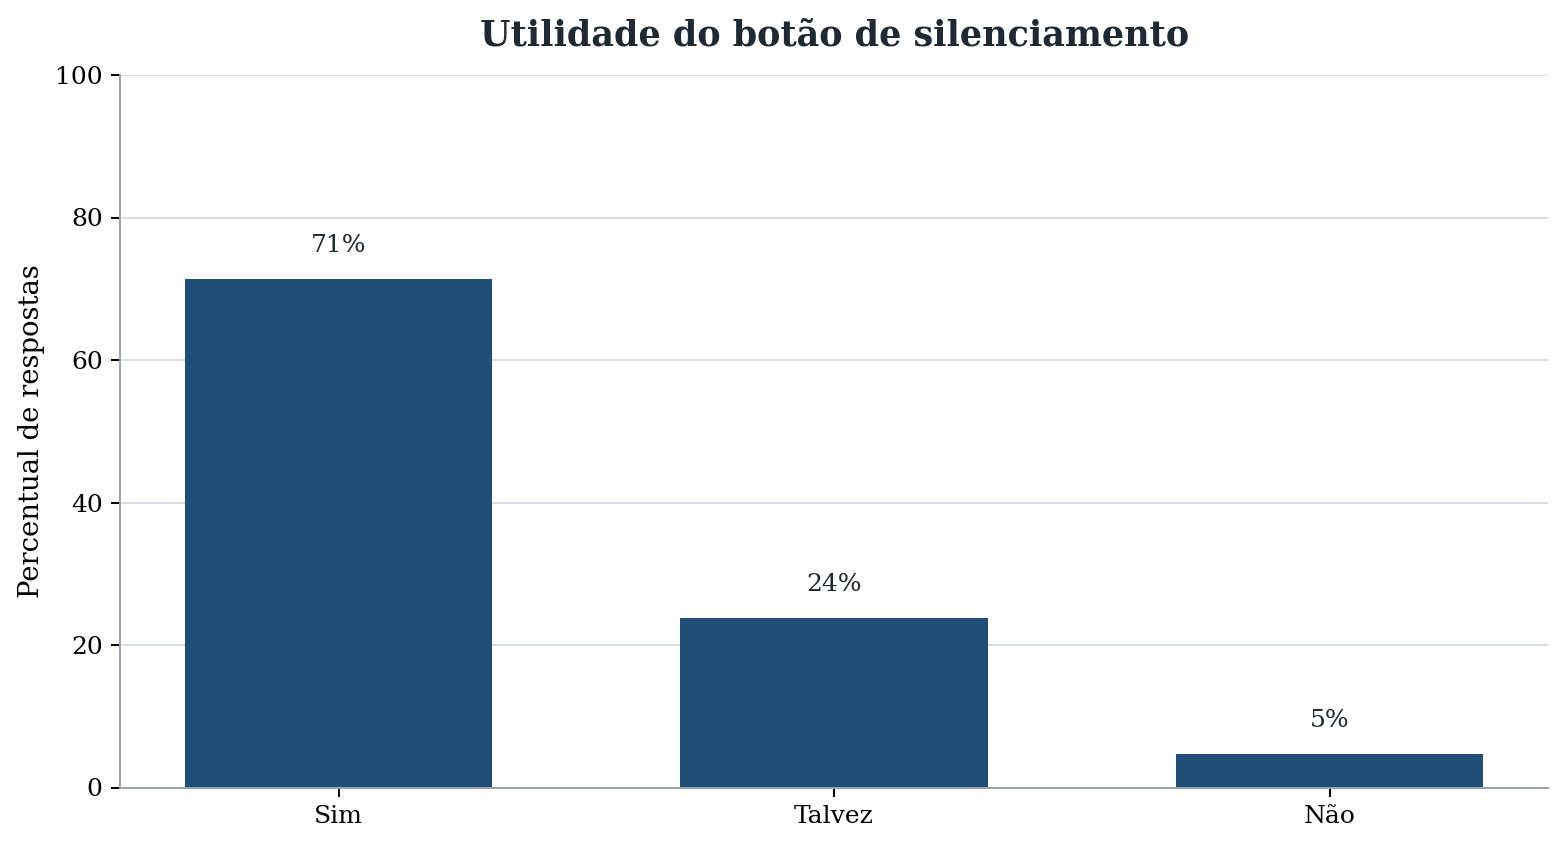
\includegraphics[width=0.78\textwidth]{figura-2.9.png}
  \caption{Utilidade de um botão para silenciar temporariamente o alarme.}
  \label{fig:2.9}
\end{figure}

\subsubsection{Local de instalação e características desejadas}

Os participantes indicaram principalmente a cozinha, o botijão e o fogão como locais relevantes para
instalação de um dispositivo de alerta. Entre as características mais citadas, destacaram-se
facilidade de instalação, aviso sonoro, baixo custo e possibilidade de integração com celular.

\begin{figure}[htbp]
  \centering
  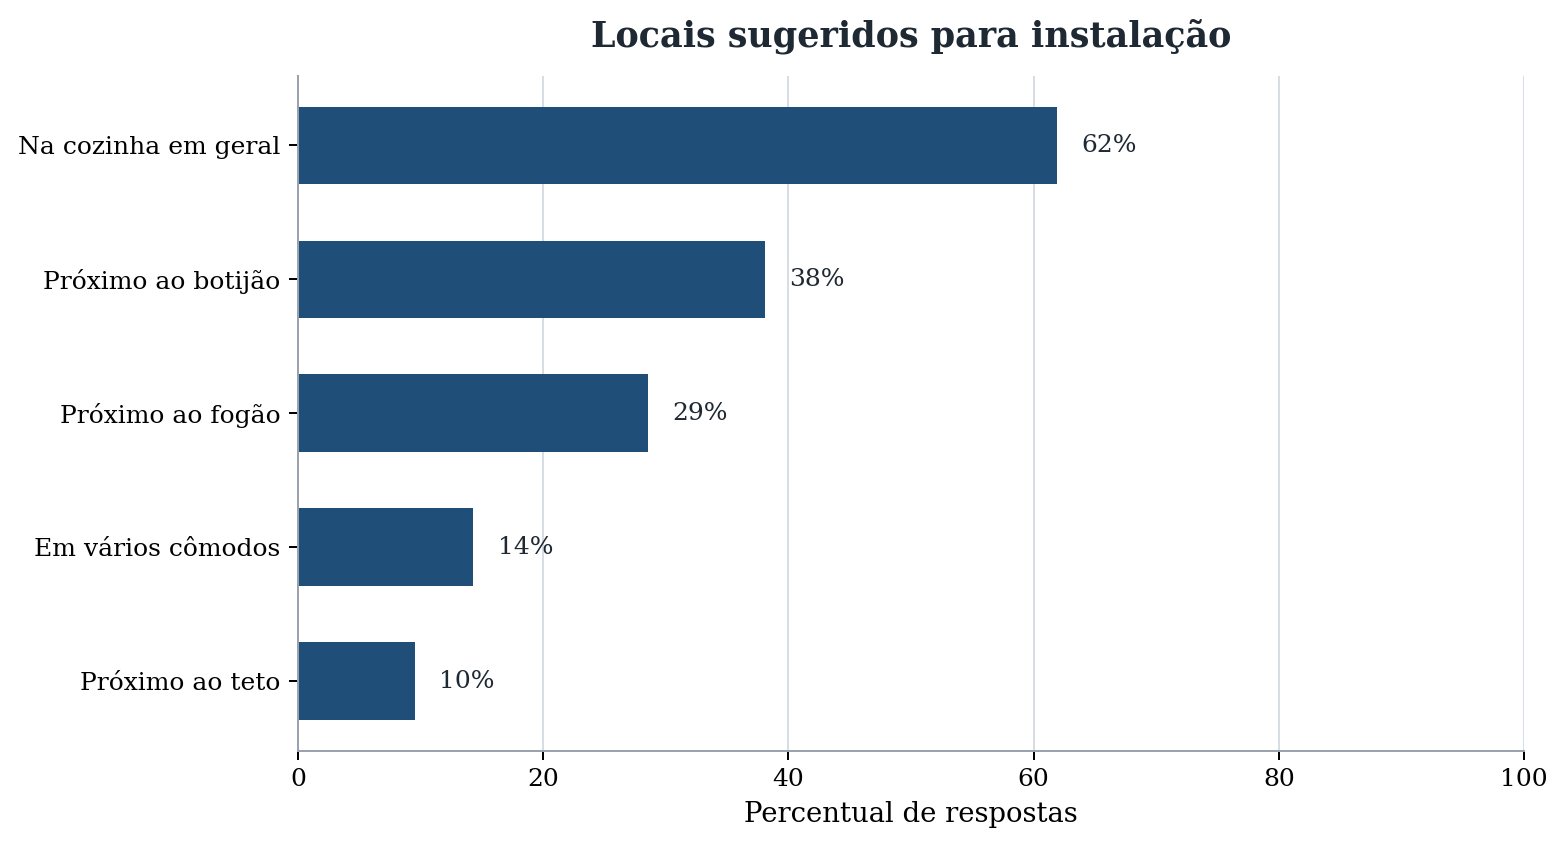
\includegraphics[width=0.78\textwidth]{figura-2.10.png}
  \caption{Locais sugeridos para instalação do dispositivo.}
  \label{fig:2.10}
\end{figure}

\begin{figure}[htbp]
  \centering
  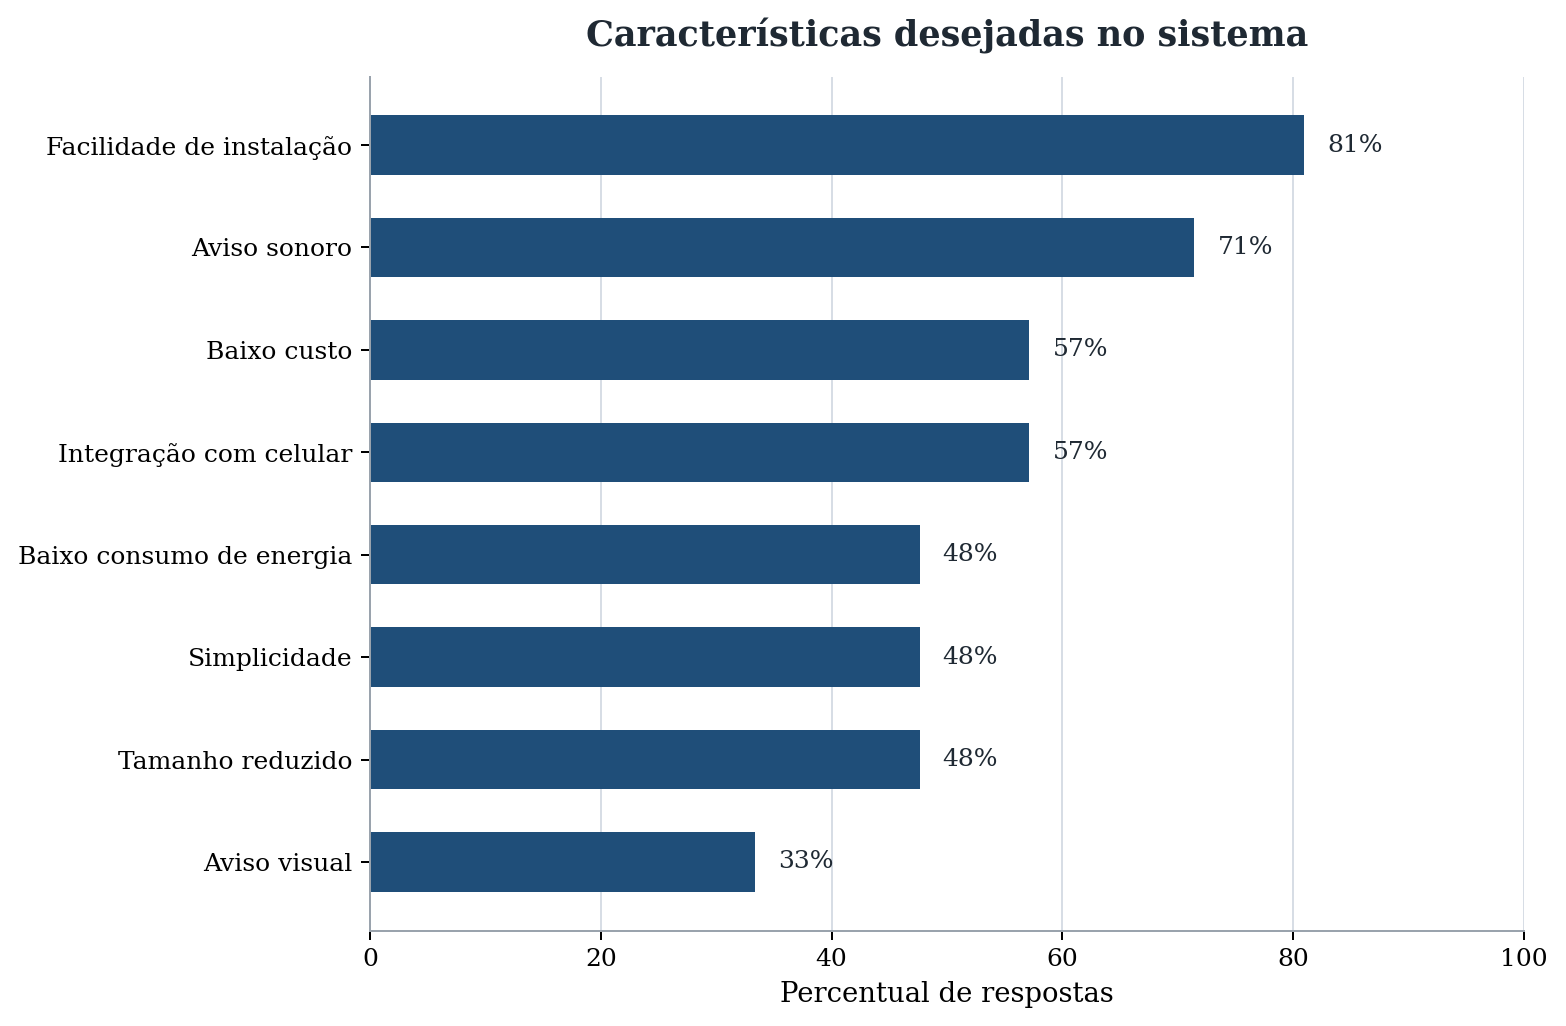
\includegraphics[width=0.78\textwidth]{figura-2.11.png}
  \caption{Características mais valorizadas em uma solução.}
  \label{fig:2.11}
\end{figure}

\subsection{Definição do problema}

Com base nas entrevistas e nos resultados do formulário digital, definiu-se como problema principal a
dificuldade de identificação rápida de vazamentos de gás em ambientes residenciais.

O problema se torna mais relevante em situações nas quais o morador depende apenas do cheiro para
perceber o vazamento, especialmente quando há limitações sensoriais, distração, ausência de pessoas
próximas ou pouca ventilação.

% =====================================================================
%  CAPÍTULO 3
% =====================================================================
\section{Proposta e Planejamento do Projeto Final}
\label{cap:proposta}

\subsection{Objetivos do trabalho}

O objetivo geral do trabalho é planejar e implementar um detector de vazamento de gás utilizando o kit
MSP430F5529LP, um sensor de gás MQ-2, um display LCD 16x2 e dispositivos de alerta.

Os objetivos específicos são:

\begin{itemize}
  \item ler o sinal analógico de um sensor de gás por meio do conversor A/D do MSP430;
  \item definir um limite de detecção para indicar possível vazamento;
  \item acionar alerta sonoro por buzzer quando o limite for ultrapassado;
  \item acionar alerta visual por LED para facilitar a percepção do evento;
  \item apresentar no LCD 16x2 o estado do sistema e o percentual da leitura em relação ao limite
        calibrado;
  \item usar o botão S2 da própria placa MSP430F5529LP para silenciamento temporário do alarme;
  \item aplicar conteúdos estudados na disciplina, principalmente GPIO, timers, interrupções, PWM,
        comunicação digital e conversão A/D;
  \item manter a montagem simples, barata e adequada para demonstração em laboratório.
\end{itemize}

\subsection{Proposta de solução}

A solução proposta é um sistema embarcado baseado na LaunchPad MSP430F5529LP. O sensor de gás MQ-2
fornecerá um sinal analógico proporcional à concentração detectada no ambiente. Esse sinal será
aplicado ao canal A0 do MSP430, disponível no pino P6.0, respeitando o limite elétrico de 3,3 V do
microcontrolador.

O MSP430 realizará leituras periódicas do sensor pelo ADC12. Quando o valor convertido ultrapassar o
limite de risco definido na calibração, o sistema interpretará a condição como possível vazamento.
Nessa situação, o microcontrolador acionará o LED1 da LaunchPad, ligado ao pino P1.0, e um buzzer
externo. O LED fornecerá alerta visual e o buzzer fornecerá alerta sonoro para que o aviso possa ser
percebido mesmo sem contato visual direto com o dispositivo.

O LCD 16x2 será usado como interface textual do protótipo. Em condição normal, o display poderá
mostrar uma mensagem como ``STATUS NORMAL'' e o percentual da leitura em relação ao limite
configurado. Em condição de alerta, o LCD poderá mostrar ``VAZAMENTO?'' e indicar que a leitura passou
de 100\% do limite. Essa indicação será útil para diferenciar uma leitura normal, uma leitura próxima
do limite e uma leitura em situação de alarme.

Também será usado o botão S2 disponível na própria LaunchPad, ligado ao pino P1.1, para silenciar
temporariamente o buzzer. O objetivo desse botão é permitir que o usuário desligue o som durante a
verificação do ambiente, sem desligar completamente o sistema. Enquanto o modo de silenciamento
estiver ativo, o LED permanecerá indicando a condição de alerta. Após o tempo definido, o alarme
sonoro voltará a ser habilitado caso o nível de gás continue acima do limite.

A proposta será organizada para utilizar conteúdos vistos na disciplina. A entrada do botão e a saída
do LED serão tratadas por GPIO; a temporização das leituras e do silenciamento será feita com timer; o
acionamento sonoro poderá usar PWM no pino P2.0/TA1.1; a leitura do MQ-2 usará o conversor A/D; a
atualização do LCD usará comunicação digital; e a resposta ao botão poderá ser feita por interrupção
externa.

\subsection{Lista de materiais e esquemático}

\subsubsection{Materiais utilizados}

\setcounter{table}{0}
\renewcommand{\thetable}{3.\arabic{table}}

\begin{table}[htbp]
  \centering
  \small
  \begin{tabular}{@{}p{3.9cm}p{6.9cm}p{3.4cm}@{}}
    \toprule
    \textbf{Componente} & \textbf{Função no projeto} & \textbf{Custo estimado} \\
    \midrule
    LaunchPad MSP430F5529LP & Microcontrolador principal, leitura do ADC e controle dos alertas & R\$ 150,00 \\
    \addlinespace
    Sensor de gás MQ-2 & Detecção de gás inflamável por saída analógica & R\$ 15,00 a R\$ 25,00 \\
    \addlinespace
    Buzzer ativo ou passivo & Alerta sonoro & R\$ 5,00 a R\$ 10,00 \\
    \addlinespace
    LED da LaunchPad & Alerta visual por meio do LED1 ligado ao P1.0 & Incluso na placa \\
    \addlinespace
    LCD 16x2 & Exibição do estado do sistema e do percentual relativo ao limite de gás & R\$ 15,00 a R\$ 30,00 \\
    \addlinespace
    Resistores & Adequação da tensão do sensor e apoio ao acionamento do buzzer, se necessário & R\$ 0,40 \\
    \addlinespace
    Protoboard e jumpers & Montagem e interligação dos componentes & R\$ 20,00 \\
    \bottomrule
  \end{tabular}
  \caption{Lista de materiais do protótipo.}
  \label{tab:materiais}
\end{table}

\subsubsection{Conexões elétricas}

As conexões previstas para o protótipo são apresentadas na tabela a seguir. Os pinos foram escolhidos
com base nos recursos disponíveis na LaunchPad MSP430F5529LP e nas funções alternativas do
MSP430F5529.

\begin{table}[htbp]
  \centering
  \small
  \begin{tabular}{@{}p{4.4cm}p{3.4cm}p{6.2cm}@{}}
    \toprule
    \textbf{Sinal} & \textbf{Pino sugerido no MSP430} & \textbf{Observação} \\
    \midrule
    Saída analógica do sensor & P6.0 / A0 & Entrada do ADC12 \\
    \addlinespace
    LED1 da LaunchPad & P1.0 & Saída digital já ligada ao LED da placa \\
    \addlinespace
    Buzzer & P2.0 / TA1.1 & Saída digital ou PWM via transistor de acionamento, se necessário \\
    \addlinespace
    Botão S2 da LaunchPad & P1.1 & Entrada digital com pull-up interno e interrupção de porta \\
    \addlinespace
    LCD 16x2 & P3.0 / SDA e P3.1 / SCL & Interface I2C com pull-ups em 3,3 V \\
    \addlinespace
    GND do sensor e periféricos & GND & Referência comum obrigatória \\
    \bottomrule
  \end{tabular}
  \caption{Conexões principais do sistema.}
  \label{tab:conexoes}
\end{table}

A LaunchPad disponibiliza alimentação de 3,3 V para o alvo e também uma linha de 5 V vinda do USB. O
MSP430F5529 opera com alimentação de 3,3 V na placa, portanto a entrada analógica do ADC não deve
receber tensão acima desse valor. Se o módulo do sensor de gás for alimentado em 3,3 V e sua saída
analógica não ultrapassar 3,3 V, a saída pode ser ligada diretamente ao ADC do MSP430. Caso o módulo
opere em 5 V e a saída analógica possa ultrapassar o limite do microcontrolador, deve ser usado um
divisor resistivo ou outro condicionamento de sinal para proteger o pino de entrada. O LCD 16x2 deverá
usar níveis lógicos compatíveis com 3,3 V; caso seja usado módulo I2C com pull-ups, esses resistores
devem ser ligados a 3,3 V, e não a 5 V, para proteger os pinos do MSP430.

Como exemplo, com resistor superior de 10\,k$\Omega$ e resistor inferior de 18\,k$\Omega$, uma saída
máxima de 5 V seria reduzida para:

\begin{equation}
  V_{ADC} = 5{,}0 \times \frac{18}{10 + 18} = 3{,}21\ \text{V}
  \label{eq:divisor}
\end{equation}

Esse valor fica abaixo de 3,3 V e permite usar a faixa de conversão do ADC sem exceder a tensão máxima
recomendada para o pino.

\subsection{Implementação}

\subsubsection{Configuração geral do MSP430}

O MSP430 será configurado para executar uma rotina cíclica de monitoramento. A cada período de
amostragem, o programa deverá ler a tensão do sensor de gás pelo ADC12, comparar o resultado com um
limite de detecção e atualizar os atuadores de alerta.

Os periféricos previstos são:

\begin{itemize}
  \item GPIO para o LED1 de alerta no pino P1.0;
  \item GPIO com interrupção para leitura do botão S2 no pino P1.1;
  \item ADC12 para leitura analógica do sensor de gás MQ-2;
  \item Timer para temporização das leituras, temporização do silenciamento e geração do sinal do
        buzzer quando aplicável;
  \item PWM no pino P2.0/TA1.1 para gerar o sinal sonoro no buzzer passivo, caso esse modelo seja usado;
  \item interface I2C para atualização do LCD 16x2.
\end{itemize}

\subsubsection{Configuração do ADC}

O conversor A/D será configurado para ler o canal A0, associado ao pino P6.0. A referência de tensão
considerada será a alimentação de 3,3 V. Como o ADC12 possui resolução de 12 bits, o resultado da
conversão varia de 0 a 4095.

A relação entre a tensão lida no pino e o valor digital convertido é:

\begin{equation}
  N_{ADC} = \frac{V_{ADC}}{V_{REF}} \times 4095
  \label{eq:adc}
\end{equation}

Considerando $V_{REF} = 3{,}3\ \text{V}$, cada unidade digital representa aproximadamente:

\begin{equation}
  \Delta V = \frac{3{,}3}{4095} = 0{,}000805\ \text{V}
  \label{eq:resolucao}
\end{equation}

Ou seja, cada contagem do ADC corresponde a cerca de 0,805 mV. Se, durante a calibração, for escolhido
um limite de alerta equivalente a 1,65 V na entrada do ADC, o valor digital correspondente será:

\begin{equation}
  N_{\text{limite}} = \frac{1{,}65}{3{,}3} \times 4095 \approx 2048
  \label{eq:nlimite}
\end{equation}

Esse limite deve ser ajustado na bancada a partir de duas medições: a leitura do sensor em ar normal e
a leitura quando o sensor é exposto a uma pequena concentração de gás em condição controlada. Para
reduzir falsos disparos, a decisão de alarme pode ser tomada pela média de várias amostras
consecutivas.

\subsubsection{Cálculo do percentual exibido}

O LCD não será usado para indicar concentração certificada em ppm, pois isso exigiria calibração
específica do sensor MQ-2, controle das condições ambientais e curva de resposta do fabricante. Para o
escopo do protótipo, será exibido um percentual relativo ao limite definido na calibração. Dessa
forma, o usuário poderá visualizar se a leitura está distante, próxima ou acima do ponto de disparo
configurado.

Primeiro, o sistema calculará a média de um conjunto de amostras do ADC:

\begin{equation}
  N_{\text{médio}} = \frac{N_1 + N_2 + \cdots + N_k}{k}
  \label{eq:media}
\end{equation}

Em seguida, o percentual em relação ao limite será calculado por:

\begin{equation}
  P_{gas} = \frac{N_{\text{médio}}}{N_{\text{limite}}} \times 100
  \label{eq:percentual}
\end{equation}

Com $N_{\text{limite}} = 2048$, uma leitura média de 1536 resultaria em:

\begin{equation}
  P_{gas} = \frac{1536}{2048} \times 100 = 75\%
  \label{eq:p75}
\end{equation}

Nesse caso, o LCD poderia indicar ``GAS: 75\% LIM'' e ``STATUS NORMAL''. Se a leitura média fosse
2560, o cálculo seria:

\begin{equation}
  P_{gas} = \frac{2560}{2048} \times 100 = 125\%
  \label{eq:p125}
\end{equation}

Nesse segundo caso, o LCD poderia indicar ``GAS:125\% LIM'' e ``VAZAMENTO?''. O alarme seria acionado
porque a leitura ultrapassou 100\% do limite calibrado.

\subsubsection{Temporização das leituras}

Para evitar leituras muito rápidas e instáveis, o sensor deverá ser lido periodicamente. Considerando
o clock SMCLK em 1 MHz e um divisor de 8 no timer, a frequência efetiva do contador fica:

\begin{equation}
  f_{\text{timer}} = \frac{1\ \text{MHz}}{8} = 125\ \text{kHz}
  \label{eq:ftimer}
\end{equation}

Com essa frequência, cada incremento do timer dura:

\begin{equation}
  T_{\text{tick}} = \frac{1}{125000} = 8\ \mu\text{s}
  \label{eq:tick}
\end{equation}

Para obter uma interrupção a cada 100 ms, o valor de comparação necessário é:

\begin{equation}
  \text{CCR0} = \frac{100\ \text{ms}}{8\ \mu\text{s}} - 1 = 12499
  \label{eq:ccr0}
\end{equation}

Assim, a cada 100 ms o sistema pode iniciar uma nova leitura do ADC. Esse intervalo é suficiente para
um detector de gás residencial, pois o fenômeno monitorado não exige resposta em microssegundos e a
média de leituras ajuda a estabilizar a decisão.

\subsubsection{Atualização do LCD 16x2}

O LCD 16x2 será atualizado em intervalos maiores que o período de amostragem do ADC, por exemplo a
cada 500 ms. Essa escolha evita atualizações excessivas no display e deixa a informação mais legível.
A primeira linha do LCD será usada para indicar o percentual relativo ao limite, enquanto a segunda
linha indicará o estado do sistema.

As mensagens planejadas são:

\begin{itemize}
  \item ``GAS: 75\% LIM'' e ``STATUS NORMAL'', quando a leitura estiver abaixo do limite;
  \item ``GAS: 98\% LIM'' e ``PROXIMO LIMITE'', quando a leitura estiver próxima do limite;
  \item ``GAS:125\% LIM'' e ``VAZAMENTO?'', quando a leitura ultrapassar o limite;
  \item ``GAS:125\% LIM'' e ``SOM SILENCIADO'', quando o buzzer estiver temporariamente desligado pelo
        botão S2.
\end{itemize}

Como o display possui apenas 16 caracteres por linha, as mensagens serão curtas e objetivas. A
atualização do LCD será tratada como uma tarefa de saída do sistema, separada da rotina crítica de
leitura do sensor e acionamento dos alertas.

\subsubsection{Acionamento do buzzer}

O buzzer será utilizado como alerta sonoro. Caso seja usado um buzzer ativo, bastará aplicar nível
lógico alto ao pino de controle para emitir som. Caso seja usado um buzzer passivo, o timer poderá
gerar uma onda quadrada por PWM no pino P2.0, que possui a função alternativa TA1.1.

Para um tom audível de aproximadamente 2 kHz usando SMCLK de 1 MHz, o período desejado é:

\begin{equation}
  T = \frac{1}{2000} = 0{,}5\ \text{ms}
  \label{eq:periodo}
\end{equation}

Logo, o valor de período do timer é:

\begin{equation}
  \text{CCR0} = \frac{1\ \text{MHz}}{2000} - 1 = 499
  \label{eq:ccr0buzzer}
\end{equation}

Para uma razão cíclica de 50\%, o registrador de comparação do PWM fica:

\begin{equation}
  \text{CCR1} = \frac{\text{CCR0} + 1}{2} = 250
  \label{eq:ccr1}
\end{equation}

O buzzer deve ser acionado por transistor quando a corrente necessária for maior que a corrente
segura do pino do MSP430.

\subsubsection{Botão de silenciamento}

O botão de silenciamento será o botão S2 disponível na própria LaunchPad, ligado ao pino P1.1. Ele
será configurado como entrada digital com resistor de pull-up interno. Nessa configuração, o pino
permanece em nível lógico alto quando o botão está solto e vai para nível lógico baixo quando o botão
é pressionado.

Para evitar leituras falsas causadas pelo repique mecânico do botão, será prevista uma temporização de
debounce de 20 ms. Usando o mesmo timer com frequência efetiva de 125 kHz, o valor correspondente é:

\begin{equation}
  N_{\text{debounce}} = 20\ \text{ms} \times 125000 = 2500
  \label{eq:debounce}
\end{equation}

Após uma pressão válida, o buzzer deverá ser silenciado temporariamente, mas o LED continuará aceso se
o nível de gás permanecer acima do limite. Essa escolha mantém a indicação de risco mesmo quando o
aviso sonoro é interrompido.

\subsection{Resultados e conclusão}

\subsubsection{Funcionamento esperado}

O protótipo deverá realizar a leitura analógica do sensor de gás, comparar o valor convertido com um
limite de alerta e acionar os dispositivos de aviso quando a leitura indicar possível vazamento. Em
condição normal, o LED deverá permanecer apagado, o buzzer desligado e o LCD deverá indicar estado
normal. Quando o valor do ADC ultrapassar o limite configurado, o LED acenderá, o buzzer será acionado
e o LCD indicará a condição de possível vazamento.

O botão de silenciamento deverá permitir a interrupção temporária do aviso sonoro durante a verificação
do ambiente. Mesmo nesse estado, o LED permanecerá indicando que o sistema ainda detecta condição de
risco e o LCD deverá mostrar que o som foi silenciado. Dessa forma, o usuário poderá reduzir o incômodo
sonoro sem perder a indicação visual e textual do problema.

\subsubsection{Atendimento esperado aos objetivos}

A solução deverá atender aos objetivos propostos porque reduz a dependência exclusiva do olfato na
identificação de vazamentos. O sistema transformará a presença de gás em um evento detectável
eletronicamente e fornecerá alertas sonoro e visual, que foram formas de aviso valorizadas na pesquisa
com a comunidade.

O projeto também deverá atender ao objetivo da disciplina de aplicar microcontroladores a um problema
prático. Serão utilizados conceitos de GPIO, interrupções, timers, PWM, conversão A/D, comunicação
digital, comparação de limiares, cálculo de média e acionamento de atuadores. Além disso, o sensor de
gás e o LCD representam interfaces externas diferentes dos dispositivos básicos usados nos exercícios
de laboratório.

\subsubsection{Limitações}

A principal limitação do protótipo é a necessidade de calibração do sensor. Sensores da família MQ
dependem de aquecimento, condições ambientais e ajuste do limiar para apresentar respostas mais
confiáveis. Por isso, o valor de alerta deve ser definido experimentalmente, comparando a leitura em
ar limpo com a leitura em uma situação controlada de presença de gás.

Outra limitação é que o sistema proposto não inclui notificação pelo celular. Embora esse recurso
tenha aparecido como característica desejável na pesquisa com a comunidade, ele exigiria um módulo
adicional de comunicação, como Wi-Fi, Bluetooth ou GSM. Esses módulos aumentariam o custo, o consumo
de energia e a complexidade da implementação, o que vai contra a proposta inicial de manter o projeto
simples e de baixo custo.

Também há limitações relacionadas à instalação física. Para uso real em uma residência, seria
necessário desenvolver uma caixa de proteção adequada, definir melhor o posicionamento próximo ao
fogão ou ao botijão e validar se o volume do alarme e a visibilidade do LED são suficientes para o
público identificado na pesquisa.

\subsubsection{Conclusão}

Conclui-se que o detector de gás com MSP430 é uma solução simples e viável para aumentar a segurança
residencial. Embora não substitua equipamentos comerciais certificados, o protótipo demonstra como um
sistema embarcado pode contribuir para alertar moradores sobre uma situação de risco e responder a uma
necessidade real identificada na comunidade.

% =====================================================================
%  DOCUMENTOS RELACIONADOS
% =====================================================================
\section*{Documentos relacionados}
\addcontentsline{toc}{section}{Documentos relacionados}

\begin{table}[htbp]
  \centering
  \small
  \begin{tabular}{@{}p{5.6cm}p{8.4cm}@{}}
    \toprule
    \textbf{Documento} & \textbf{Conteúdo} \\
    \midrule
    \texttt{docs/engenharia.md} & Arquitetura, pinagem, condicionamento de sinal e fórmulas \\
    \addlinespace
    \texttt{docs/pesquisa.md} & Pesquisa de campo ampliada, com os números reais \\
    \addlinespace
    \texttt{docs/figures/README.md} & Mapeamento das figuras originais e dos gráficos analíticos \\
    \addlinespace
    \texttt{docs/BUGS\_E\_MELHORIAS.md} & Bugs encontrados e melhorias planejadas \\
    \addlinespace
    \texttt{hardware/lista-de-materiais.md} & Lista de materiais (BOM) detalhada \\
    \addlinespace
    \texttt{hardware/diagrama.svg} & Diagrama de ligação e arquitetura do sistema \\
    \bottomrule
  \end{tabular}
  \caption*{Documentação complementar do repositório.}
\end{table}

\end{document}
